% Metódy inžinierskej práce

\documentclass[10pt,twoside,slovak,a4paper]{article}

\usepackage[slovak]{babel}

\usepackage[IL2]{fontenc} 
\usepackage[utf8]{inputenc}
\usepackage{graphicx}
\usepackage{url} 
\usepackage{hyperref} 

\usepackage{cite}



\title{{\bf Modelovanie spracovania elektronického podania ÚPVS sekvenčnými UML diagramami}\thanks{Semestrálny projekt v predmete Metódy inžinierskej práce, ak. rok 2021/22, vedenie: Vladimír Mlynarovič}}

\author{Viktor Uhlár\\[2pt]
	{\small Slovenská technická univerzita v Bratislave}\\
	{\small Fakulta informatiky a informačných technológií}\\
	{\small \texttt{xuhlar@stuba.sk}}
	}

\date{\small 14. November 2021} 


\linespread{1.2}
\begin{document}



\begin {titlepage}
\centering
\maketitle

\begin{abstract}


\noindent{Ústredný portál verejnej správy (ÚPVS) je centrálnym miestom na podávanie a spracovanie elektronických podaní. Pre agendové informačné systémy poskytuje možnosť integrácie tak, aby bolo možné zasielať elektronické podania priamo z vlastných informačných systémov (teda bez nutosti priuhlasovania sa do elektronických schránok pomocou eID - elektronického občianskeho preukazu).}\newline
\noindent{Keďže postupnosť spracovania elektronického podania závisí od jeho účelu, musí byť pred fázou samotnej integrácie vypracovaný model ``workflow“. ÚPVS pre tento účel vyžaduje tzv. Dohodu o integračnom zámere, kde je spracovanie modelované vo forme sekvenčného UML diagramu.
V tejto práci sa teda budem venovať teórii modelovania sekvenčných UML modelov s konrétnym príkladom pre spracovanie elektronického rozhodnutia ``fiktívneho“  OVM (orgánu verejnej moci SR).}

\end{abstract}

\end{titlepage}
\flushleft
\section{Úvod}\label{1sek}

Ústredný portál verejnej správy (ÚPVS) je centrálnym miestom na podávanie a spracovanie elektronických podaní. Umožňuje vykonávať elektronickú úradnú komunikáciu s ktorýmkoľvek orgánom verejnej moci a nasmeruje používateľa na využitie konkrétnej elektrickej služby verejnej správy. Pre agendové informačné systémy poskytuje možnosť integrácie tak, aby bolo možné pristupovať k elektronickej schránke priamo z vlastných informačných systémov - teda bez nutnosti prihlasovania sa eID - elektronického občianskeho preukazu.\cite{UPVS}\cite{SVK.sk} \\

Keďže spôsob pripojenia môže byť rôzny, správca ÚPVS (Národná agentúra pre sieťové a elektronické služby - NASES) vyžaduje podrobný integračný zámer, ktorého súčasťou je aj modelovanie integrácie vo forme sekvenčného UML diagramu.\newline



V tejto práci sa teda budem venovať:

\begin{itemize}
\item Rámcovému popisu UML a typov diagramov \ref{2sek}
\item Spôsobu tvorby sekvenčných UML diagramov \ref{3sek}
\item Príkladu UML integračného diagramu pre UPVS \ref{4sek}
\end{itemize}

Informácie pre vytvorenie tejto práce som čerpal:

\begin{itemize}
\item Z integračnej dokumentácie spoločnosti NASES
\item Z internetových zdrojov ku UML modelovaniu
\item Z praktickej skúsenosti pri spolupráci v rámci integračného ÚPVS projektu
\end{itemize}
Zoznam konkrétnej použitej literatúry je uvedený v prílohe Literatúra.\\

Práca môže byť užitočná nielen pre analytikov, ktorí zodpovedajú za modelovanie integračných ``ÚPVS“ projektov, ale aj pre všeobecnejšie pochopenie zmyslu sekvenčných diagramov (ako integrálnej súčasti software development cyklov).




\section{Popis UML a rozdelenie typov diagramov} \label{2sek}

UML znamená Unified Modeling Language, teda grafický jazyk na vizualizáciu, špecifikáciu, navrhovanie a dokumentáciu programových systémov. 

UML ponúka štandardný spôsob zápisu tak návrhov systémov vrátane konceptuálnych prvkov ako sú business procesy a systémové funkcie, tak konkrétnych prvkov ako sú príkazy programovacieho jazyka, databázové schémy a znovupoužiteľné programové komponenty.\cite{WIKI}\newpage

Pomocou UML je možné modelovať niekoľko rozličných diagramov. Ich charakteristika je zrejmá z nasledovného obrázku\ref{TypyD}:


\begin{figure}[h]
\centering
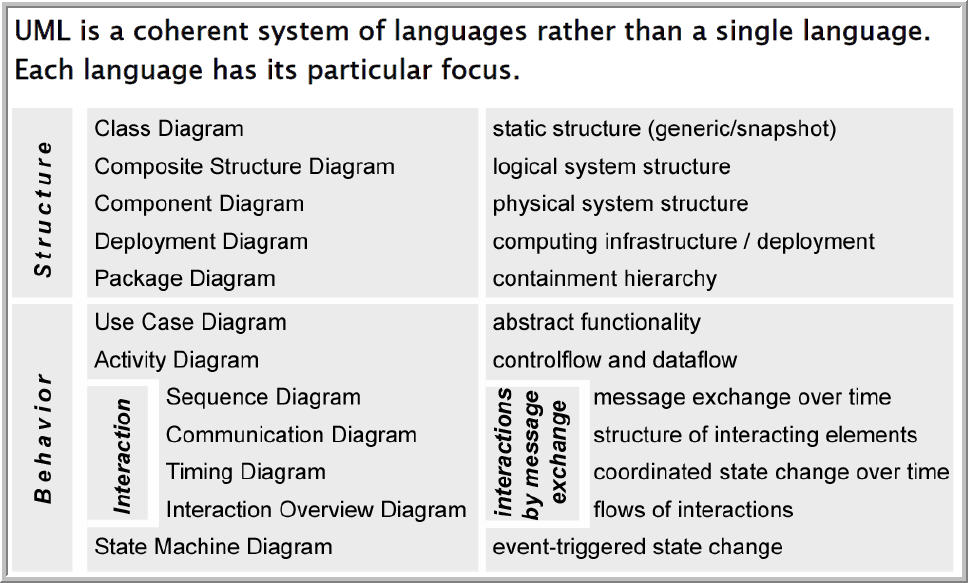
\includegraphics[width=0.75\textwidth]{Images/Obr1.jpg}
\caption{Typy diagramov\cite{UMLUni}}
\label{TypyD}
\end{figure}

 Diagramy je teda možné rozdeliť do 3 základných skupín\cite{WIKI}:

\begin{enumerate}
\item Štruktúrne diagramy, kam patria:
	\begin{itemize}
	\item diagram tried (class diagram)
	\item diagram komponentov (component diagram)
	\item diagram zloženej štruktúry (composite structure diagram)
	\item diagram nasadenia (deployment diagram)
	\item diagram balíčkov (package diagram)
	\item diagram objektov (object diagram), nazýva sa aj diagram inštancií
	\end{itemize}
\item Diagramy správania, kam patria:
	\begin{itemize}
	\item diagram aktivít (activity diagram)
	\item diagram prípadov použitia (use case diagram)
	\item stavový diagram (state machine diagram)
	\end{itemize}

\item Diagramy interakcie, kam patria:
	\begin{itemize}
	\item sekvenčný diagram (sequence diagram)
	\item diagram komunikácie (communication diagram) - predtým diagram spolupráce (collaboration diagram)
	\item diagram prehľadu interakcií (interaction overview diagram)
	\item diagram časovania (timing diagram)
	\end{itemize}
\end{enumerate}



\section{Sekvenčný diagram a jeho modelovanie} \label{3sek}

Sekvenčný diagram modeluje interakciu medzi objektami počas konkrétneho ``use case“, teda prípadu použitia. Graficky ilustruje, ako rozličné časti systému navzájom spolupracujú tak, aby zrealizovali požadovanú funkciu.\ref{Strukt} Zjednodušene povedané: sekvenčný diagram ukazuje postup činností rozličných častí systému\cite{SDT}.\newline

Pri zobrazení sa využívanie niekoľko značiek, pričom k najpoužívanejším patria\ref{tabulka}:
\begin{table}[h!]
\centering
\caption{Vysvetlenie daných značiek\cite{TabJa}}
\label{tabulka}
\resizebox{0.55\textwidth}{!}{%
\begin{tabular}{|l|l|}
\hline
\multicolumn{1}{c}{Značka} & \multicolumn{1}{c}{Význam} \\ \hline
Lifeline                   & životná línia              \\ \hline
Actor                      & účinkujúci                 \\ \hline
Activity                   & aktivita                   \\ \hline
State                      & stav                       \\ \hline
Message arrow              & tok informácie     \\ \hline
\end{tabular}%
}
\end {table}


Na nasledovnom obrázku je ilustrácia jednoduchého sekvenčného diagramu, využívajúceho vyššie uvedené značky\cite{SDT}:
\begin{figure}[h]
\centering
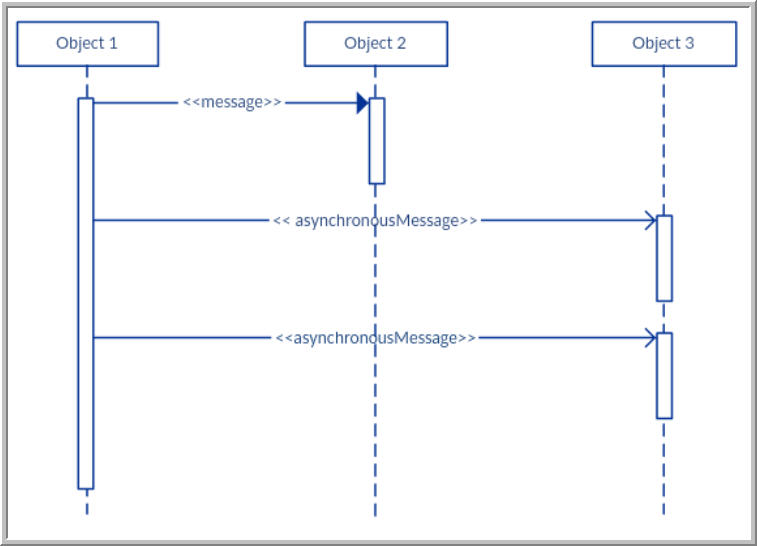
\includegraphics[width=0.75\textwidth]{Images/Obr2.jpg}
\caption{Priklad štruktúry sekvenčného diagramu\cite{SDT}}
\label{Strukt}
\end{figure}



\section{Príklad UML integračného diagramu pre UPVS} \label{4sek}

\begin{figure}[h!]
\centering
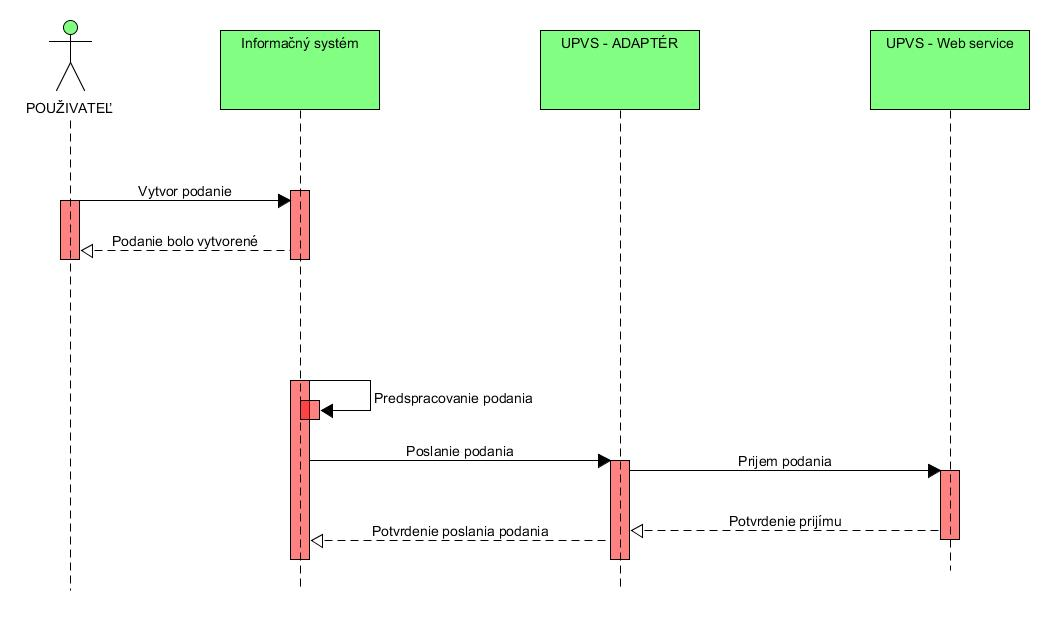
\includegraphics[width=\textwidth]{Images/Obr3.jpg}
\caption{Prikladný model pripojenia informačného systému k ÚPVS\cite{UMLetJa}}
\label{Model}
\end{figure}

Na nižšie uvedenom obrázku sa nachádza konkrétny príklad modelu - sekvenčného UML diagramu, ktorý popisuje spôsob pripojenie informačného systému daného ministerstva ku ÚPVS. Model zobrazuje štyri základné objekty, medzi ktorými prebieha tok údajov:
\begin{description}
\item a)        Používateľ informačného systému
\item b)        Informačný systém (najčastejšie pre správu registratúry)
\item c)        bezpečnostný ÚPVS adaptér, vytvárajú zabezpečený komunikačný kanál
\item d)        samotný ÚPVS portál so svojimi modulmi
\end{description}
Šípky v UML diagrame predstavujú časovo synchronizované komunikačné kroky, ktoré zabezpečujú odoslanie údajov zo vstupného formulára (podania) do elektronickej schránky adresáta na ÚPVS a následne potvrdenie o úpešnosti realizácie tejto operácie.\newline



\newpage
\section{Vyjadrenia na témy z prednášok} \label{5sek}


\paragraph{Spoločenské súvislosti informatiky}

Motiváciou pôsobiť v tejto oblasti je vzťah ku programovaniu a využitím IT technológií možnosť ``kultivovať“ prácu používateľov. Zvlášť ma zaujíma ``human-computer“ interakcia – teda vytvárania ergonomicky správneho GUI.

\paragraph{Technológia a ľudia.}

Problémom tvorby informačných systémov je nejednosť v predstave o ich funkčnosti medzi používateľom, sponzorom (teda tým kto ho financuje) a tvorcom (software inžinierom). Každý z nich má o tej istej veci rôznu predstavu. Tak ako dodať technologické riešenie tak, aby bol súlad výsledku s predstavou na začiatku čo najbližší?

\noindent Odpoveďou je agilný resp. tzv.  ``scrum“ prístup – teda tvorba systému v krokových iteráciach, kedy si ich používateľ priebežne overuje vytvorenú verziu systému a operatívne ``usmerňuje“ smer jej ďalšieho vývoja.

\paragraph{Udržateľnosť a etika.}

Činnosť v oblasti software inžinierstva sa zdá na prvý pohľad ``odtrhnutá“ od otázok udržateľného rozvoja spoločnosti. No po hlbšej analýze sa ukáže, že produkt tejto činnosti – informačné systémy – zásadne vplývajú na správanie sa ich používateľov. 

\noindent Rozvoj digitalizácie spôsobuje stále väčší vplyv na život spoločnosti. Tento fakt otvára mnohé etické otázky, ktoré popisuje dokument ``Software Engineering Code of Ethics and Professional Practice“, kde sú popísané princípy ``príkladného správania“ pre sofware inžiniersto. Patrí tam napr. zohľadnenie záujmov používateľa, dôraz na profesionalitu pri tvorbe produktu, kooperácia s kolegami či celoživotné vzdelávanie.


\section{Zhodnotenie} \label{6sek} 
Zmyslom tejto práce bolo charakterizovať modelovanie komunikácie v informačných systémoch pomocou sekvenčných UML diagramov a popísať konkrétny príklad, ktorý bol použitý pri projekte pripojenia informačného systému ministerstva ku ÚPVS.
Tieto informácie môžu poslúžiť členom projektových tímov, ktorí sa ocitnú pred podobnou „integračnou“ výzvou – či už voči ÚPVS alebo ku inému systému. \\

\newpage




\bibliography{Uhlar_Literatura}
\bibliographystyle{abbrv} 
\end{document}
